%%%%%%%%%%%%%%%%%%%%%%%%%%%%% Define Article %%%%%%%%%%%%%%%%%%%%%%%%%%%%%%%%%%
\documentclass{article}
%%%%%%%%%%%%%%%%%%%%%%%%%%%%%%%%%%%%%%%%%%%%%%%%%%%%%%%%%%%%%%%%%%%%%%%%%%%%%%%

%%%%%%%%%%%%%%%%%%%%%%%%%%%%% Using Packages %%%%%%%%%%%%%%%%%%%%%%%%%%%%%%%%%%
\usepackage{geometry}
\usepackage{graphicx}
\usepackage{caption}
\usepackage{subcaption}
\usepackage{amssymb}
\usepackage{amsmath}
\usepackage{amsthm}
\usepackage{empheq}
\usepackage{mdframed}
\usepackage{booktabs}
\usepackage{lipsum}
\usepackage{graphicx}
\usepackage{color}
\usepackage{psfrag}
\usepackage{pgfplots}
\usepackage{bm}
\usepackage{float}
\usepackage{physics}
\usepackage{hyperref}
\usepackage{xcolor}
\usepackage{titlesec}
\usepackage{algorithmic}
\hypersetup{
	colorlinks=true,
	linkcolor=blue,
	filecolor=magenta,
	urlcolor=cyan
}
\usepackage{animate}
\usepackage{svg}
% Quantum physics inner product
\newcommand{\innerp}[2]{\left\langle #1 \vert #2 \right\rangle}
\newcommand{\convolution}[2]{(#1 \star #2)}

%%%  \begin{figure}[htp]
%%%  	\centering
%%%  	\includegraphics[width=0.25\textwidth]{/path/to/image}
%%%  	\caption{}\label{fig:}
%%%  \end{figure}

% to write multiple lines of equations

%%  \begin{align*}
%%  \begin{split}
%%  	\ket{\phi} + \ket{\psi} &= \ket{\phi + \psi} \\
%%  	a \ket{\psi} &= \ket{a \psi}
%%  \end{split}
%%  \end{align*}

\newcommand{\e}[1]{\times 10^{#1}}

\usepackage{listings}
\lstset{showstringspaces=false} % pretty embeded code in LaTeX
%%%%%%%%%%%%%%%%%%%%%%%%%%%%%%%%%%%%%%%%%%%%%%%%%%%%%%%%%%%%%%%%%%%%%%%%%%%%%%%

% Other Settings

%%%%%%%%%%%%%%%%%%%%%%%%%% Page Setting %%%%%%%%%%%%%%%%%%%%%%%%%%%%%%%%%%%%%%%
\geometry{a4paper}

%%%%%%%%%%%%%%%%%%%%%%%%%% Define some useful colors %%%%%%%%%%%%%%%%%%%%%%%%%%
\definecolor{ocre}{RGB}{243,102,25}
\definecolor{mygray}{RGB}{243,243,244}
\definecolor{deepGreen}{RGB}{26,111,0}
\definecolor{shallowGreen}{RGB}{235,255,255}
\definecolor{deepBlue}{RGB}{61,124,222}
\definecolor{shallowBlue}{RGB}{235,249,255}
%%%%%%%%%%%%%%%%%%%%%%%%%%%%%%%%%%%%%%%%%%%%%%%%%%%%%%%%%%%%%%%%%%%%%%%%%%%%%%%

%%%%%%%%%%%%%%%%%%%%%%%%%% Define an orangebox command %%%%%%%%%%%%%%%%%%%%%%%%
\newcommand\orangebox[1]{\fcolorbox{ocre}{mygray}{\hspace{1em}#1\hspace{1em}}}
%%%%%%%%%%%%%%%%%%%%%%%%%%%%%%%%%%%%%%%%%%%%%%%%%%%%%%%%%%%%%%%%%%%%%%%%%%%%%%%

%%%%%%%%%%%%%%%%%%%%%%%%%%%% English Environments %%%%%%%%%%%%%%%%%%%%%%%%%%%%%
\newtheoremstyle{mytheoremstyle}{3pt}{3pt}{\normalfont}{0cm}{\rmfamily\bfseries}{}{1em}{{\color{black}\thmname{#1}~\thmnumber{#2}}\thmnote{\,--\,#3}}
\newtheoremstyle{myproblemstyle}{3pt}{3pt}{\normalfont}{0cm}{\rmfamily\bfseries}{}{1em}{{\color{black}\thmname{#1}~\thmnumber{#2}}\thmnote{\,--\,#3}}
\theoremstyle{mytheoremstyle}
\newmdtheoremenv[linewidth=1pt,backgroundcolor=shallowGreen,linecolor=deepGreen,leftmargin=0pt,innerleftmargin=20pt,innerrightmargin=20pt,]{theorem}{Theorem}[section]
\theoremstyle{mytheoremstyle}
\newmdtheoremenv[linewidth=1pt,backgroundcolor=shallowBlue,linecolor=deepBlue,leftmargin=0pt,innerleftmargin=20pt,innerrightmargin=20pt,]{definition}{Definition}[section]
\theoremstyle{myproblemstyle}
\newmdtheoremenv[linecolor=black,leftmargin=0pt,innerleftmargin=10pt,innerrightmargin=10pt,]{problem}{Problem}[section]
%%%%%%%%%%%%%%%%%%%%%%%%%%%%%%%%%%%%%%%%%%%%%%%%%%%%%%%%%%%%%%%%%%%%%%%%%%%%%%%

%%%%%%%%%%%%%%%%%%%%%%%%%%%%%%% Plotting Settings %%%%%%%%%%%%%%%%%%%%%%%%%%%%%
\usepgfplotslibrary{colorbrewer}
\pgfplotsset{width=8cm,compat=1.9}
%%%%%%%%%%%%%%%%%%%%%%%%%%%%%%%%%%%%%%%%%%%%%%%%%%%%%%%%%%%%%%%%%%%%%%%%%%%%%%%

%% Centering section titles
\titleformat{\section}[block]{\Large\bfseries\filcenter}{}{1em}{}

%% norm
%%\newcommand\norm[1]{\lVert #1 \rVert}


\title{Machine learning - random}
\author{Aheer Srabon}
\date{}

\begin{document}
\maketitle

\section{Section 1}
\noindent The linear unit works as follows in Keras,

\begin{figure}[htp]
	\centering
	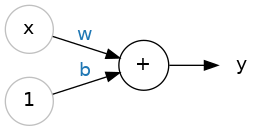
\includegraphics[width=0.3\textwidth]{../assets/machine_learning_random/the_linear_unit.png}
	\caption{The linear unit: $ y = wx + b $.}
\end{figure}

\begin{figure}[htp]
	\centering
	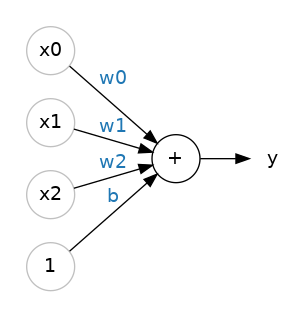
\includegraphics[width=0.3\textwidth]{../assets/machine_learning_random/a_linear_unit_with_multiple_inputs.png}
	\caption{A linear unit with three inputs - $ y = w_0 x_0 + w_1 x_1 + w_2 x_2 + b $}
\end{figure}

\pagebreak

% Using TensorFlow keras
\begin{lstlisting}[language=Python]
from tensorflow import keras
from tensorflow.keras import layers

# Create a network with 1 linear unit
model = keras.Sequential([
	layers.Dense(units=1, input_shape=[3])
])
\end{lstlisting}

\noindent keras.Sequential creates a neural network as a stack
of layers. The above example defines a model accepting three input
features and producing a single output. The first argument units
define how many outputs we want. The second argument input\_shape
tells keras the dimensions of the input. input\_shape is the number
of columns of the DataFrame except for the output column. It is a
python list to permit use of more complex datasets.

\noindent Neural networks typically organize their neurons into layers.
When we collect together linear units having a common set of inputs, we
get a \textbf{dense} layer.

\begin{figure}[htp]
	\centering
	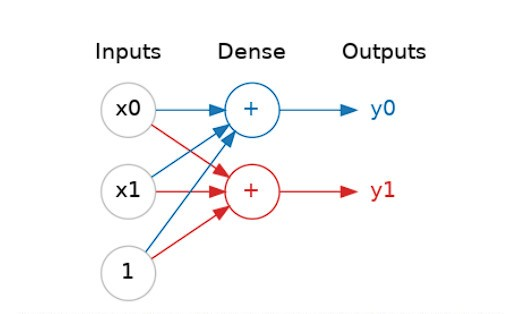
\includegraphics[width=0.5\textwidth]{../assets/machine_learning_random/denser_layer_with_two_inputs_and_a_bias.jpg}
	\caption{A dense layer of two linear units receiving two inputs and a bais.}
\end{figure}

\noindent Each layer in neural network performs some kind of relatively
simple transformation. Through a deep stack of layers, a neural network can
transform its inputs in more and more complex ways. In a well-trained
neural network, each layer is a transformation getting us a little bit
closer to a solution. A "layer" in Keras is a very general kind of thing.
A layer can be, essentially, any kind of data transformation (like
convolution, recurrence). 

\subsection{The activation function}
\noindent It turns out that two dense layers with nothing in between
are no better than a single dense layer by itself. \emph{Dense layers by
themselves can never move us out of the world of lines and planes.}
An activation function brings non-linearity to the model. An 
\textbf{activation function} is simply some function that is applied to
each of a layer's outputs (its activations). The most common is the
rectifier function $ max(0,x) $. When a attach a rectifier to a linear
unit, we get a rectified linear unit or \textbf{ReLU}. Applying a ReLU
activation to a linear unit means the output becomes $ max(0, wx + b) $,
which might be drawn like:

\begin{figure}[htp]
	\centering
	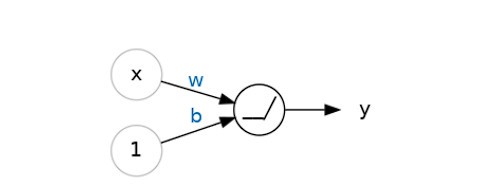
\includegraphics[width=0.5\textwidth]{../assets/machine_learning_random/rectified_linear_unit.jpg}
	\caption{A rectified linear unit.}
\end{figure}

\noindent Stacking dense layers,

\begin{figure}[htp]
	\centering
	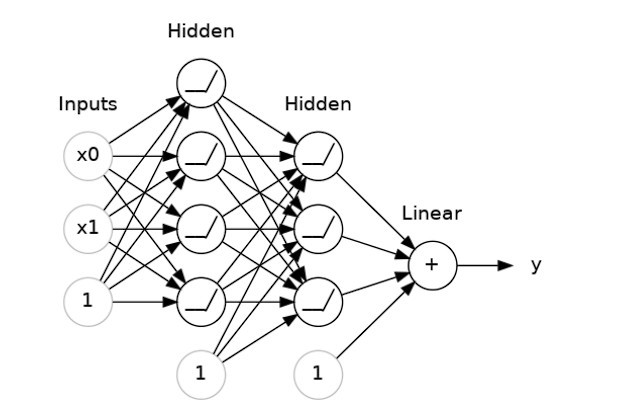
\includegraphics[width=0.5\textwidth]{../assets/machine_learning_random/stack_of_dense_layers.jpg}
	\caption{A stack of dense layers makes a "fully-connected" network.}
\end{figure}

\noindent The final (output) layer is a linear unit (with no activation function).
That makes this network appropriate to a \emph{regression}, task. Other tasks (like
classification) might require an activation function on the output.

\subsection{Building sequential models}
The Sequential model we've been using will connect together a list of layers
in order from first to last: the first layer gets the input, the last layer
produces the output. This creates the model in the figure above:

\begin{lstlisting}[language=Python]
from tensorflow import keras
from tensorflow.keras import layers

model = keras.Sequential([
    # the hidden ReLU layers
    layers.Dense(units=4, activation='relu', input_shape=[2]),
    layers.Dense(units=3, activation='relu'),
    # the linear output layer 
    layers.Dense(units=1),
])
\end{lstlisting}

\noindent Sequential takes a list of layers. Sometimes, some other
layer are put between the Dense layer and its activation function. In
these cases, the activation can be defined on its own Activation layer.

\begin{lstlisting}[language=Python]
from tensorflow import keras
from tensorflow.keras import layers

model = keras.Sequential([
    # the hidden ReLU layers
    layers.Dense(units=4, activation='relu', input_shape=[2]),
    layers.Dense(units=3)
    # The activation is in its own layer. Between
    # the Dense layer and the Activation layer, some other layers can be 
    # put
    layers.Activation('relu')
    # the linear output layer 
    layers.Dense(units=1),
])
\end{lstlisting}

\noindent To train a neural network, the following things are needed,
\begin{itemize}
	\item The model iteself
	\item Training data
	\item A loss function (tells the network what problem to solve)
	\item An optimizer (tells the network how to solve the problem)
\end{itemize}

\noindent Some example of loss functions are,
\begin{itemize}
	\item Mean Absolute Error (MAE)
	\item Mean Squared Error (MSE)
	\item Huber loss
\end{itemize}

\subsection{Stochastic gradient descent}
\noindent Virtually all of the optimization algorithms used in deep learning
belong to a family called \textbf{stochastic gradient descent}. They are
iterative algorithms that train a network in steps.
\begin{enumerate}
	\item Sample some training data and run it through the network to make
		predictions
	\item Measure the loss between the predictions and the true values
	\item Finally, adjust the weights in a direction that makes the loss smaller
\end{enumerate}

\noindent Repeat the above process until the loss as small as necessary (or until
it won't decrease any further). Each iteration's sample of training data is called
a \textbf{minibatch} (or often just "batch"), while a complete round of the training data
is called an \textbf{epoch}. A smaller learning rate means the network needs to see
more \textbf{minibatches} before its weights converge to their best value.
The number of epochs you train for is how many times the network will see each
training example. \emph{The learning rate and the size of the minibatches are the two
parameters that have the largest effect on how the SGD training proceeds.}

\noindent \textbf{Stochastic} means "determined by chance". The training is stochastic
because the minibatches are random samples from the dataset.

\noindent A common loss function for regression problems is \textbf{mean absolute
error} or \textbf{MAE}.

\begin{figure}[htp]
	\centering
	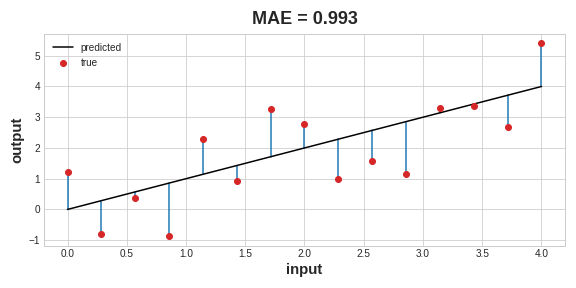
\includegraphics[width=0.5\textwidth]{../assets/machine_learning_random/mean_absolute_error.png}
	\caption{The mean absolute error is the average length between the fitted curve and the data points.}
\end{figure}

\noindent The loss function tells the network its objective. The optimizer is an
algorithm that adjusts the weights of the model to minimize the loss. The learning rate
and the size of the minibatches are the two parameters that have the largest effect
on how the SGD training proceeds.

\noindent \textbf{Adam} is an SGD algorithm that has an adaptive learning rate that
makes it suitable for most problems without any parameter tuning. Adam is a great general
purpose optimizer. After defining a model, a loss function and optimzer with the models
compile method can be defined,

\begin{lstlisting}[language=Python]
model.compile(
	optimzer="adam",
	loss="mae",
)
\end{lstlisting}

\noindent Splitting the data into training data and validation data,
\begin{lstlisting}[language=Python]
import pandas as pd
from IPython.display import display

red_wine = pd.read_csv('../input/dl-course-data/red-wine.csv')

# Create training and validation splits
df_train = red_wine.sample(frac=0.7, random_state=0)
df_valid = red_wine.drop(df_train.index)
display(df_train.head(4))

# Scale to [0, 1]
max_ = df_train.max(axis=0)
min_ = df_train.min(axis=0)
df_train = (df_train - min_) / (max_ - min_)
df_valid = (df_valid - min_) / (max_ - min_)

# Split features and target
X_train = df_train.drop('quality', axis=1)
X_valid = df_valid.drop('quality', axis=1)
y_train = df_train['quality']
y_valid = df_valid['quality']

_, input_shape = X_train.shape
\end{lstlisting}

\noindent Choose a three-layer network with over 1500 neurons. 

\begin{lstlisting}[language=Python]
from tensorflow import keras
from tensorflow.keras import layers

model = keras.Sequential([
    layers.Dense(512, activation='relu', input_shape=[11]),
    layers.Dense(512, activation='relu'),
    layers.Dense(512, activation='relu'),
    layers.Dense(1),
])
\end{lstlisting}

\noindent Deciding the architecture of the model should be part of the process.
Start simple and use the validation loss as guide. Compile the optimzer and loss
function,

\begin{lstlisting}[language=Python]
model.compile(
	optimizer='adam',
	loss='mae'
)
\end{lstlisting}

\noindent The following code tells Keras to feed the optimizer 256 rows of the training
data at a time (the batch\_size) and to do that 10 times all the way through the
dataset (the epochs),

\begin{lstlisting}[language=Python]
history = model.fit(
	X_train, y_train,
	validation_data = (X_valid, y_valid),
	batch_size=256,
	epochs=10,
)

# convert the training history to a dataframe
history_df = pd.DataFrame(history.history)
history_df['loss'].plot()
\end{lstlisting}

\subsection{Overfitting and Underfitting}
Information of the training data as being two kinds,
\begin{itemize}
	\item \emph{Signal} - is the part that generalizes, the part that can help
		the model to make predictions from new data. Useful.
	\item \emph{Noise} - is the part that is only true for the training data. It
		is all of the random fluctuation that comes from data in the real-world
		or all of the incidental, non-informative patterns that can't actually
		help the model make predictions. Not useful.
\end{itemize}

\begin{figure}[htp]
	\centering
	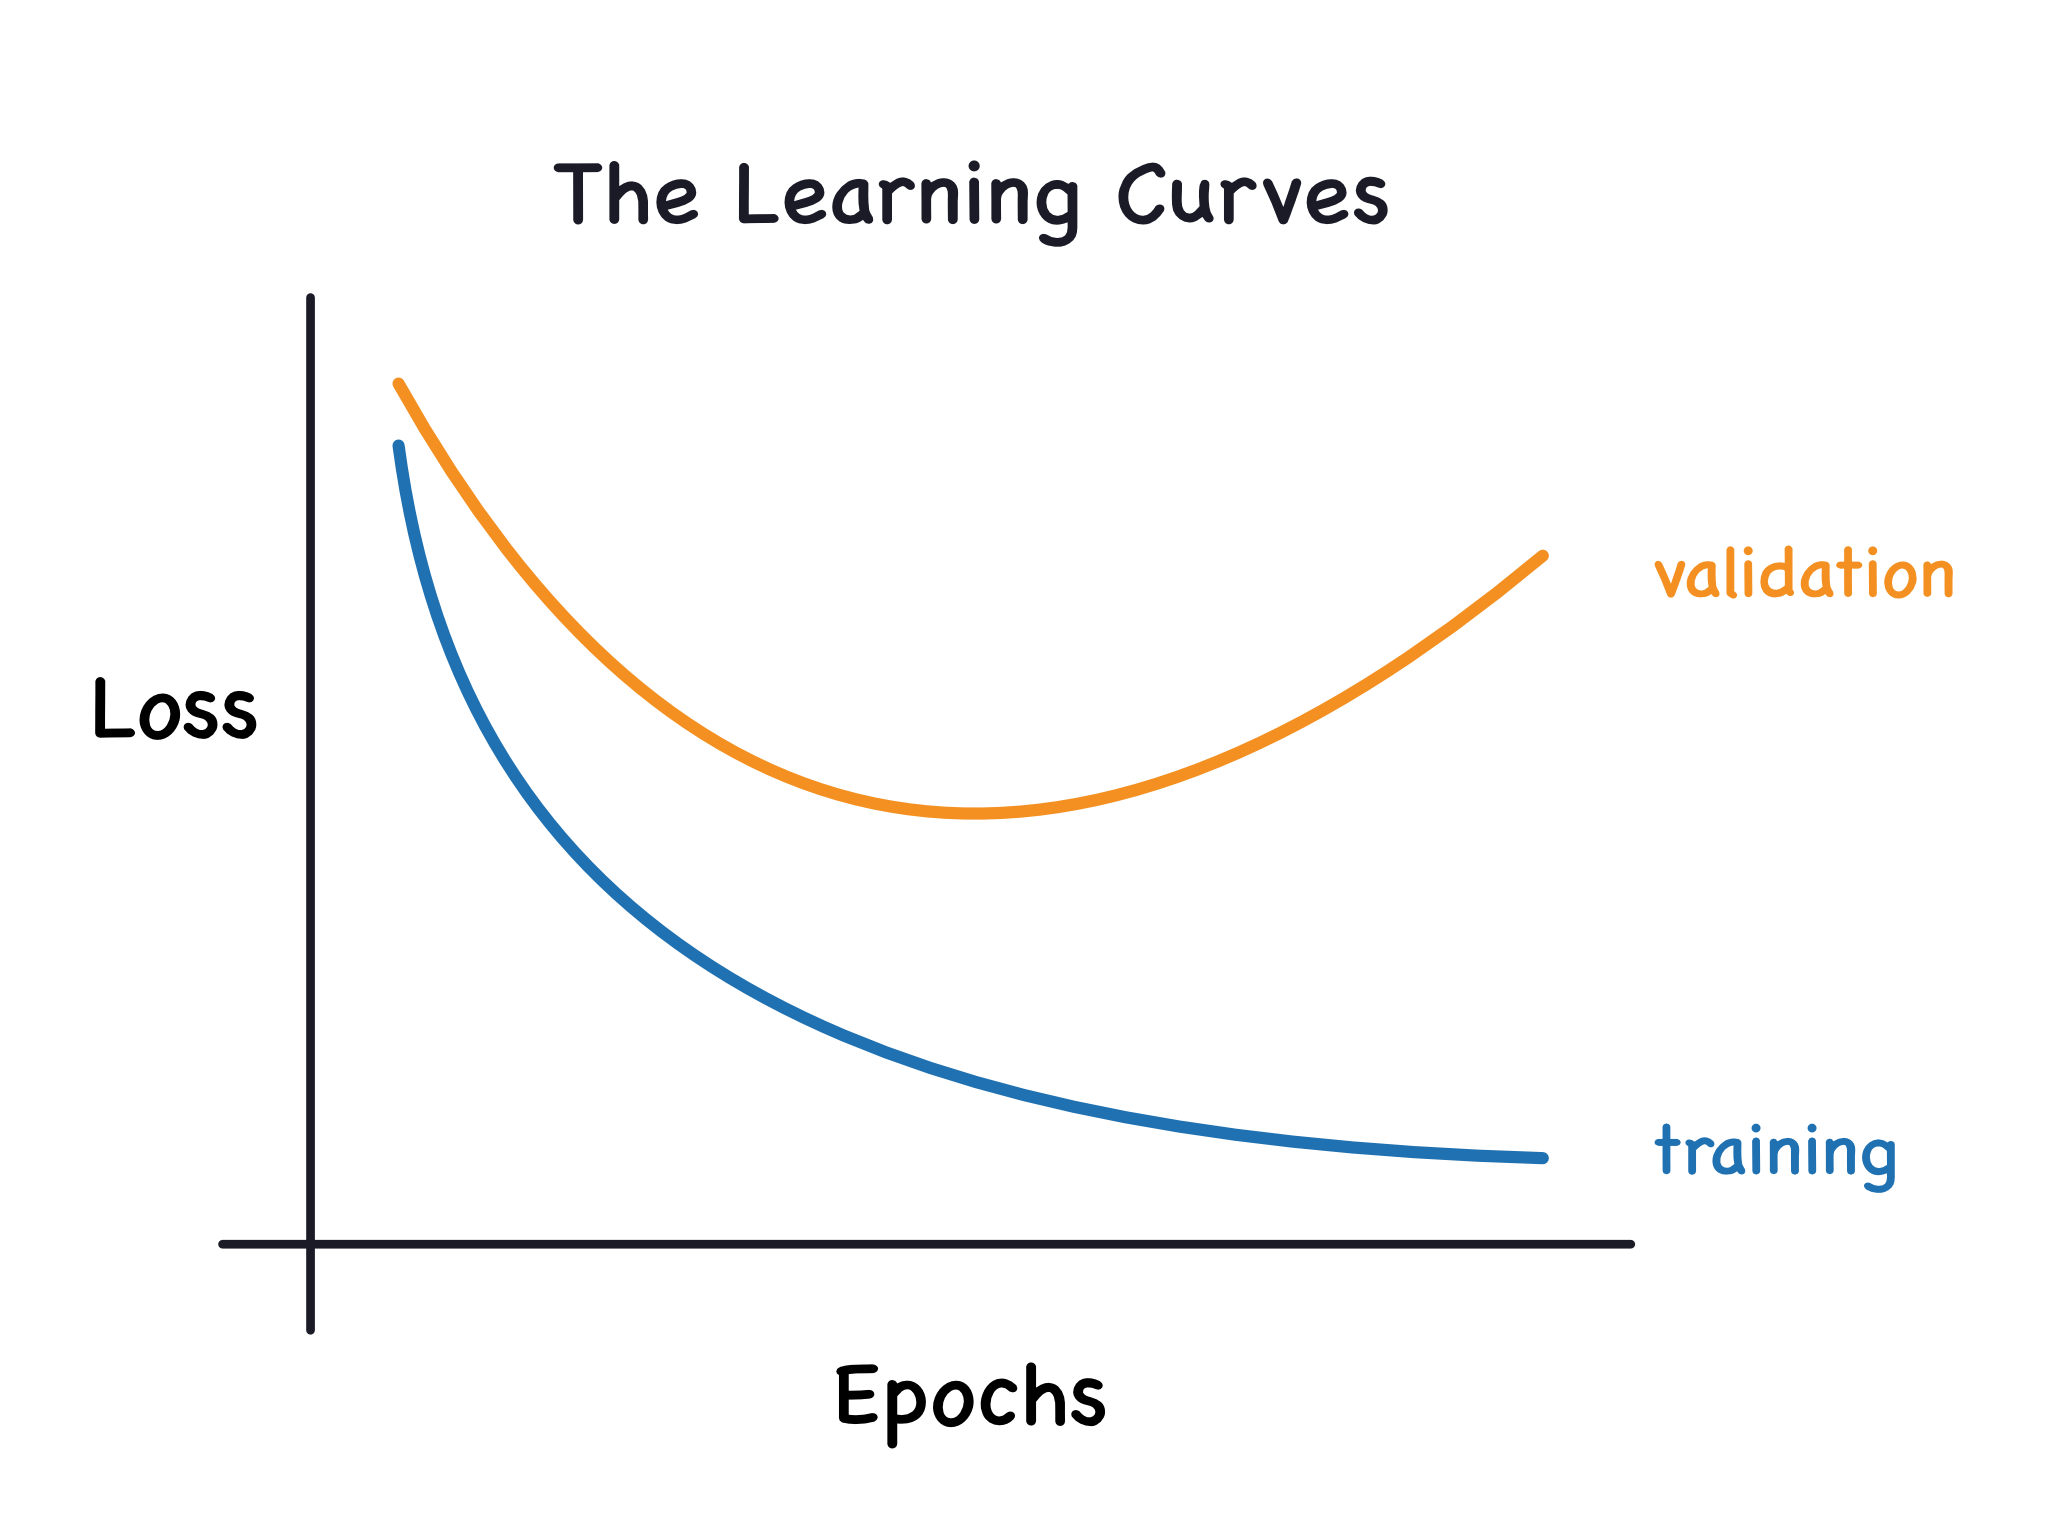
\includegraphics[width=0.5\textwidth]{../assets/machine_learning_random/signal_vs_noise.png}
	\caption{The validation loss gives an estimate of the expected error on unseen data.}
\end{figure}

\noindent The training loss will go down either when the model learns signal or when it
learns noise. But the validation loss will go down only when the model learns signal (
whatever noise the model learned from the training set won't generalize to new data). So,
when a model learns signal, both curves go down, but when it learns noise, a gap is created
in the curves. The size of the gap tells us how much noise the model has learned.

\noindent Underfitting vs overfitting,

\begin{figure}[htp]
	\centering
	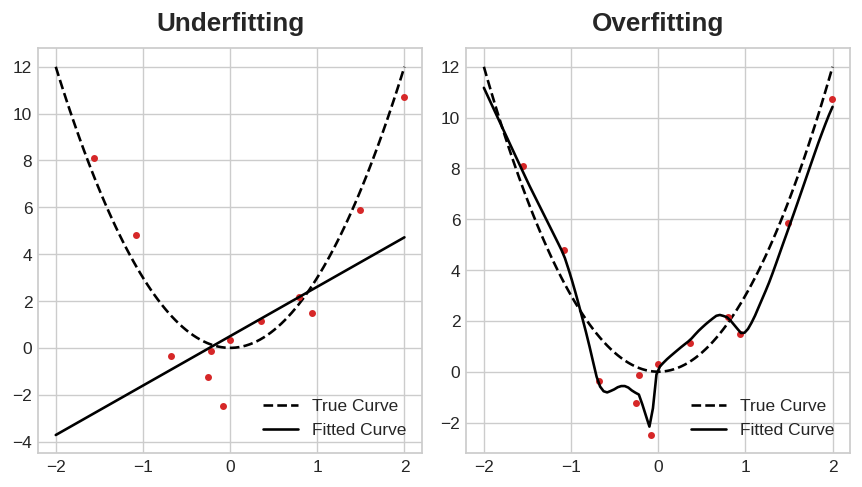
\includegraphics[width=0.5\textwidth]{../assets/machine_learning_random/underfitting_vs_overfitting.png}
	\caption{Underfitting vs overfitting}
\end{figure}

\begin{itemize}
	\item \textbf{Underfitting} the training set is when the loss is not as
		low as it could be because the model hasn't learned enough \emph{signal.}
	\item \textbf{Overfitting} the training set is when the loss is not as low
		as it could be because the model learned too much \emph{noise.}
\end{itemize}

\noindent A model's \emph{capacity} refers to the \textbf{size} and \textbf{capacity} of the
patterns it is able to learn,
\begin{itemize}
	\item Wider neural network -- more units to existing layers. Learns linear
		relationships easily
	\item Deeper neural network -- adding more layers. Learns non-linear
		relationships easily
\end{itemize}

\begin{figure}[htp]
	\centering
	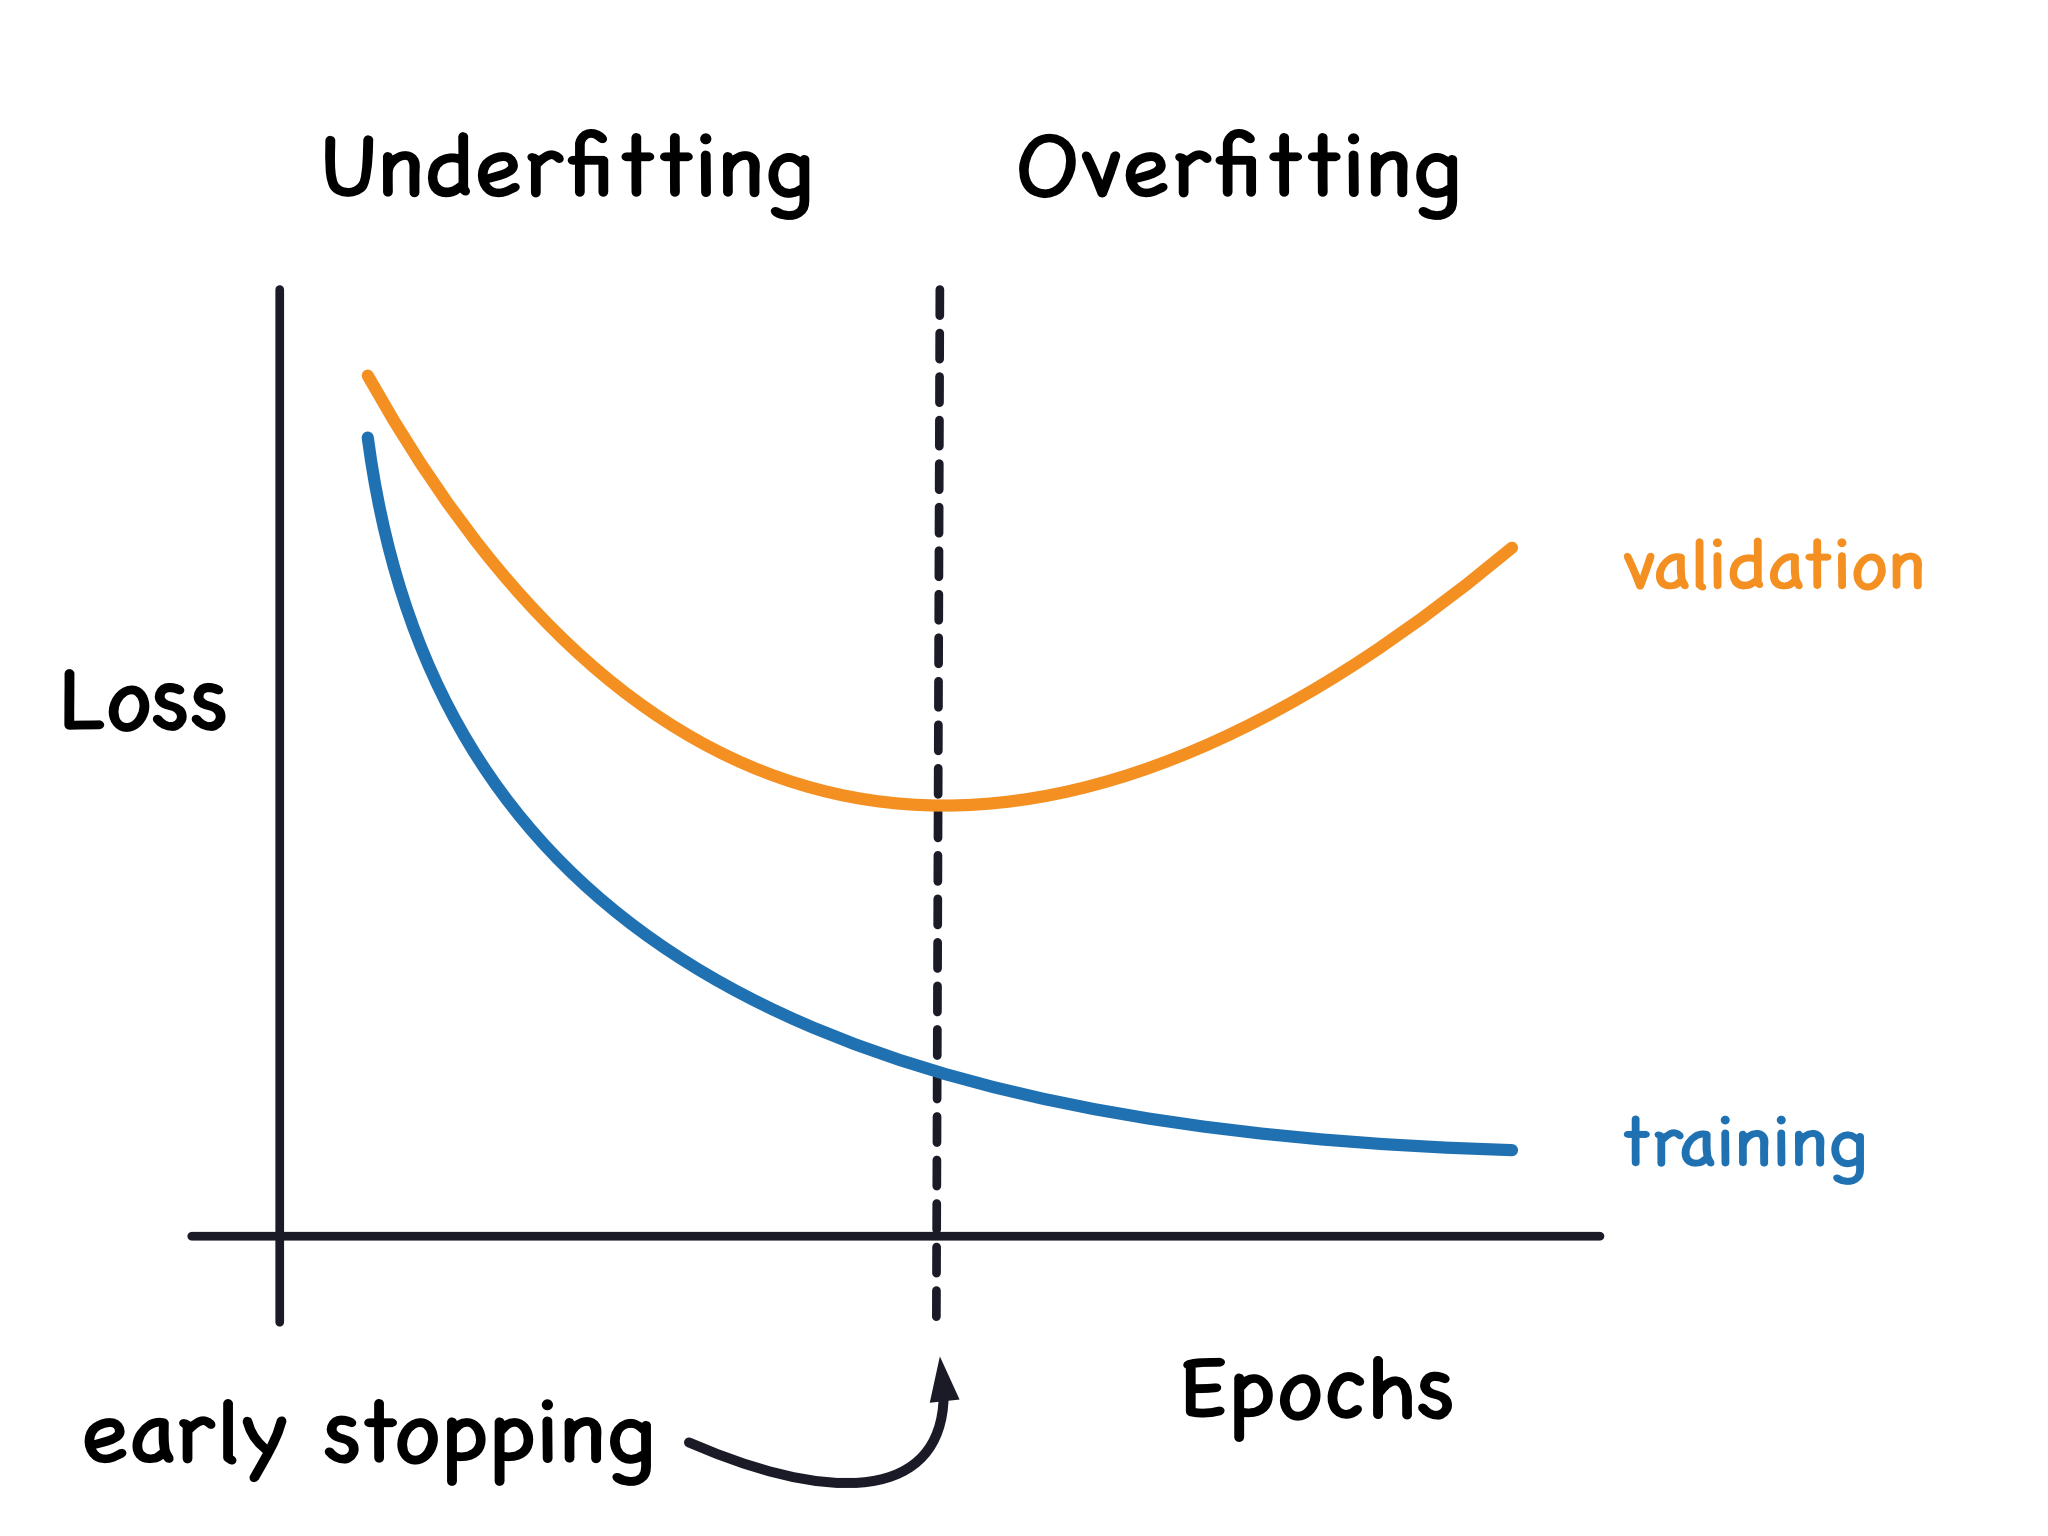
\includegraphics[width=0.5\textwidth]{../assets/machine_learning_random/early_stopping.png}
	\caption{We keep the model where the validation loss is at a minimum - early stopping}
\end{figure}

\noindent Once we detect that the validation loss is starting to rise again, we can reset
the weights back to where the minimum occured. This is called \emph{early stopping}. In
Keras, early stopping can be included through a callback. A callback is a function that is
run every so often while the network trains. The early stopping callback will run after
every epoch.

\begin{lstlisting}[language=Python]
from tensorflow.keras.callbacks import EarlyStopping

early_stopping = EarlyStopping(
    min_delta=0.001, # minimium amount of change to count as an improvement
    patience=20, # how many epochs to wait before stopping
    restore_best_weights=True,
)
\end{lstlisting}

\noindent These parameters say: "If there hasn't been at least an improvement of $ 0.001 $
in the validation loss over the previous 20 epochs, then stop the training and keep the best
model you found."

\vspace{0.5cm}
\noindent Train a neural network,

\begin{lstlisting}[language=Python]
import pandas as pd
from tensorflow import keras
from tensorflow.keras import layers, callbacks

red_wine = pd.read_csv('../input/dl-course-data/red-wine.csv')

# Create training and validation splits
df_train = red_wine.sample(frac=0.7, random_state=0)
df_valid = red_wine.drop(df_train.index)

# Scale to [0, 1]
max_ = df_train.max(axis=0)
min_ = df_train.min(axis=0)
df_train = (df_train - min_) / (max_ - min_)
df_valid = (df_valid - min_) / (max_ - min_)

# Split features and target
X_train = df_train.drop('quality', axis=1)
X_valid = df_valid.drop('quality', axis=1)
y_train = df_train['quality']
y_valid = df_valid['quality']


early_stopping = callbacks.EarlyStopping(
    min_delta=0.001, # minimium amount of change to count as an improvement
    patience=20, # how many epochs to wait before stopping
    restore_best_weights=True,
)

model = keras.Sequential([
    layers.Dense(512, activation='relu', input_shape=[11]),
    layers.Dense(512, activation='relu'),
    layers.Dense(512, activation='relu'),
    layers.Dense(1),
])
model.compile(
    optimizer='adam',
    loss='mae',
)
history = model.fit(
    X_train, y_train,
    validation_data=(X_valid, y_valid),
    batch_size=256,
    epochs=500,
    callbacks=[early_stopping], # put your callbacks in a list
    verbose=0,  # turn off training log
)

history_df = pd.DataFrame(history.history)
history_df.loc[:, ['loss', 'val_loss']].plot();
print("Minimum validation loss: {}".format(history_df['val_loss'].min()))
\end{lstlisting}

\end{document}
